\chapter{Abschlussaufgabe OAR}
OAR ist ein opensource Batchsystem. Es findet vorallem Anwendung im HPC Bereich.
Dass OAR bereit ist produktiv eingesetzt zu werden, beweist seine Benutzung in Projekten wie Grid'5000 (1000 Nodes, 8000 Cores).
\begin{figure}[H]
	\centering
	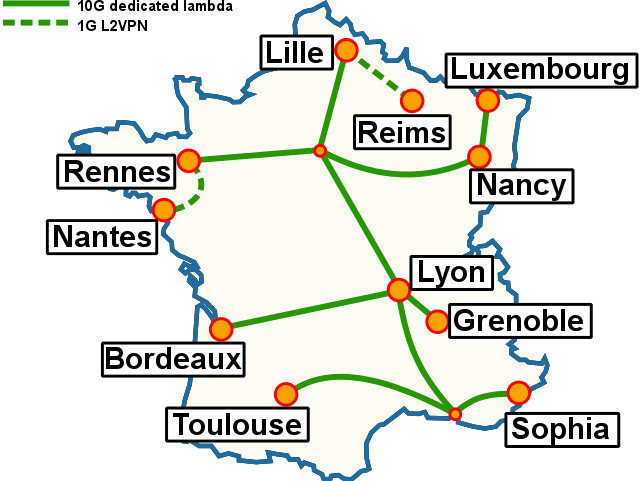
\includegraphics[scale=1.5]{grid5000.jpg} 
	\vspace{-10pt}
	\caption{Grid'5000}
\end{figure}
Zuerst wird die zugrundeliegende Architektur erklärt und die dazugehörigen Installationsschritte auf dem Debiansystem beschrieben,
da diese nicht trivial sind.
Anschließend werden Unterschiede zum Batchsystem Slurm verdeutlicht.
Zuletzt werden noch Benchmarks beider Batchsysteme gezeigt und verglichen.\pagebreak
\section{Architektur}
Eine typische OAR Installation besteht aus vier Komponenten. All diese sind im Debian Repository in der (aktuellen) Version 2.5.4-2 
zu finden:
    \begin{itemize}
        \item{Server node}
        \item{Frontend node}
        \item{Computing node}
        \item{Optional: Visualisierungsserver}
    \end{itemize}
    Debian Pakete:
    \begin{itemize}
        \item{oar-server}
        \item{oar-user}
        \item{oar-node}
    \end{itemize}

    \begin{figure}[h]
    \centering
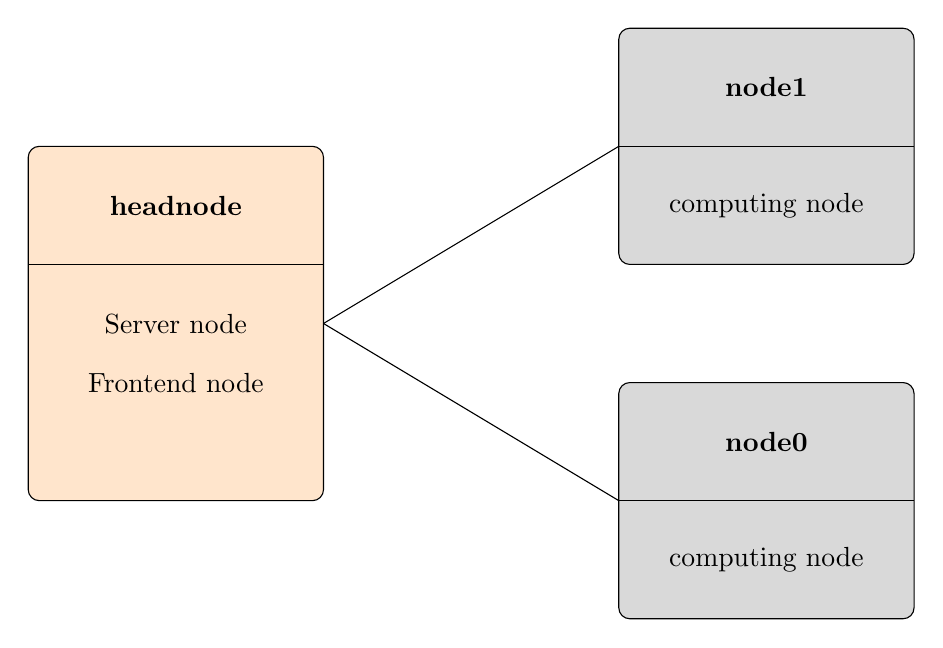
\begin{tikzpicture}[scale=1.5]
        %headnode
        \draw [rounded corners,fill=orange!20](0,1) rectangle (2.5,4); 
        \node at (1.25,3.5)[font=\bfseries] {headnode};
        \draw (0,3) -- (2.5,3);
        \node at (1.25,2.5) {Server node};
        \node at (1.25,2) {Frontend node};
        %node0
        \draw [rounded corners,fill=gray!30](5,0) rectangle (7.5,2); 
        \node at (6.25,1.5)[font=\bfseries] {node0};
        \draw (5,1) -- (7.5,1);
        \node at (6.25,0.5) {computing node};
        %node1
        \draw [rounded corners,fill=gray!30](5,3) rectangle (7.5,5); 
        \node at (6.25,4.5)[font=\bfseries] {node1};
        \draw (5,4) -- (7.5,4);
        \node at (6.25,3.5) {computing node};
        %edges
        \draw (2.5,2.5) -- (5,1);
        \draw (2.5,2.5) -- (5,4);
    \end{tikzpicture}
    \caption{Architekturskizze von OAR auf LCTP G1 Cluster} 
\end{figure}
\newpage

\section{Installation und Konfiguration}
    Auf den computenodes:
    \begin{lstlisting}[style=Bash]
    # apt-get install oar-node
	\end{lstlisting}
    Die /etc/sshd.conf auf den computenodes muss angepasst werden.
    Dieser Schritt ist in der Dokumentation auf der OAR Webseite nicht zu finden, wird aber benötigt.
    \begin{lstlisting}[style=Bash]
    AcceptEnv OAR_CPUSET OAR_JOB_USER
    PermitUserEnvironment yes
	\end{lstlisting}
    Auf dem headnode:
    \begin{lstlisting}[style=Bash]
    # apt-get install oar-server oar-server-mysql
    # oar-database --create --db-admin-user <user> -db-admin-pass <passwd>
    add nodes:
    # oarnodesetting -a -h node0
    # oarnodesetting -a -h node1
	\end{lstlisting}
\section{Benutzerinteraktion}
Der User interagiert mit dem Batchsystem auf dem Frontend Node auf ähnliche Weise wie mit Slurm. Die grundlegenden Befehle sind vergleichbar
            \begin{table}[h]
        \begin{tabular}{l|l}
          OAR command & Slurm command \\ \hline
        oarsub & sbatch  \\
        oardel  & scancel  \\
        oarstat & squeue  \\
        oarhold & scontrol suspend  \\
          oarresume & scontrol resume \\
    \end{tabular}
\end{table}\\
    Beispiel job submission: \lstinline{frontend:~> oarsub -l /cpu=2,walltime=00:30:00 ./script.sh}
	\newpage
\section{Benchmark}
	Zum Benchmarking wurde die Zeit in Abhängigkeit der Anzahl
    der schon wartenden Jobs gemessen,
    die das jeweilige Batchsystem benötigt um einen Job in die Queue einzureihen.\\
	\begin{figure}[H] \centering
		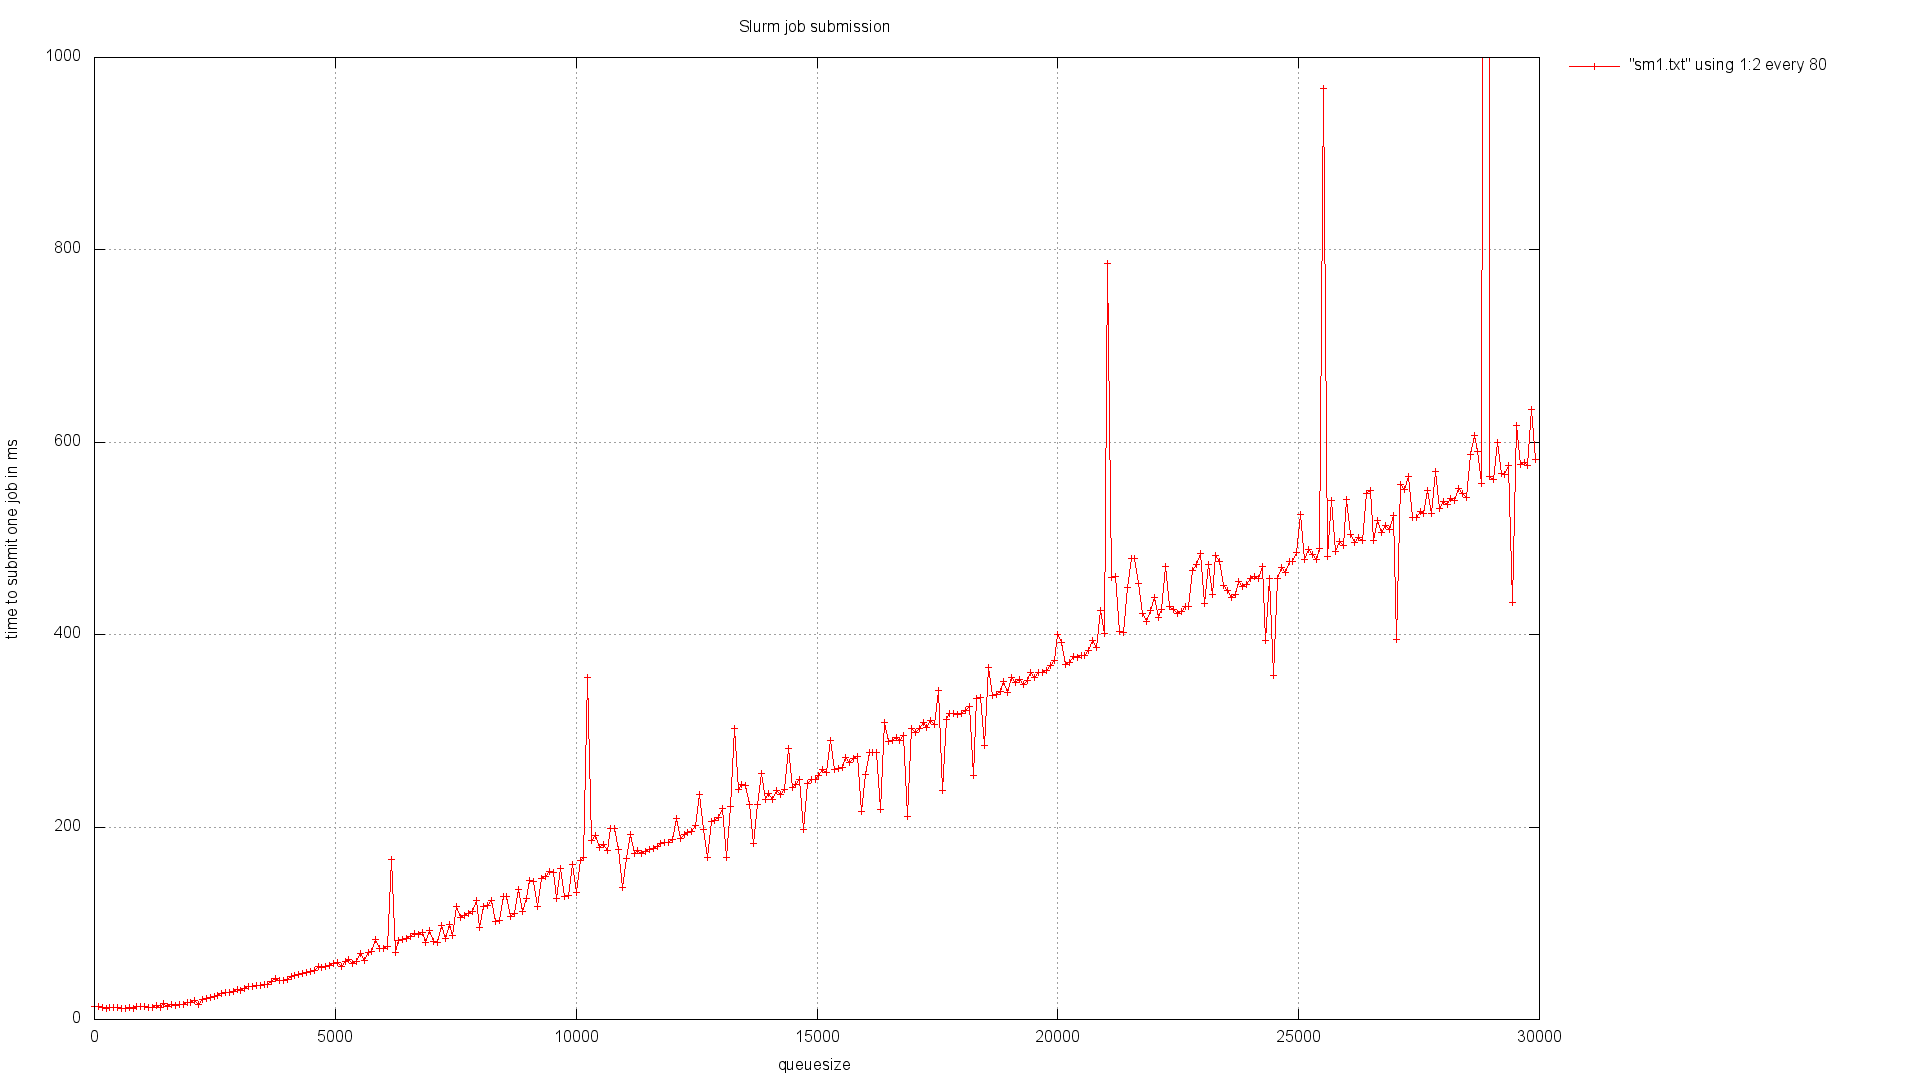
\includegraphics[scale=0.8]{../oar/output/pics/slurm.png} 
		\caption{Slurm submission time}
	\end{figure}
    Bei Slurm ist zu erkennen, dass bis ca. 2000 wartender Jobs die Zeit, die 
    benötigt wird einen Job in die Queue einzureihen bei ~15ms liegt. 
    Ab 2000 Jobs steigt diese Zeit jedoch. Bei 30000 Jobs liegt die Zeit schon
    über 600ms
	\newpage

	\begin{figure}[H]
		\centering
		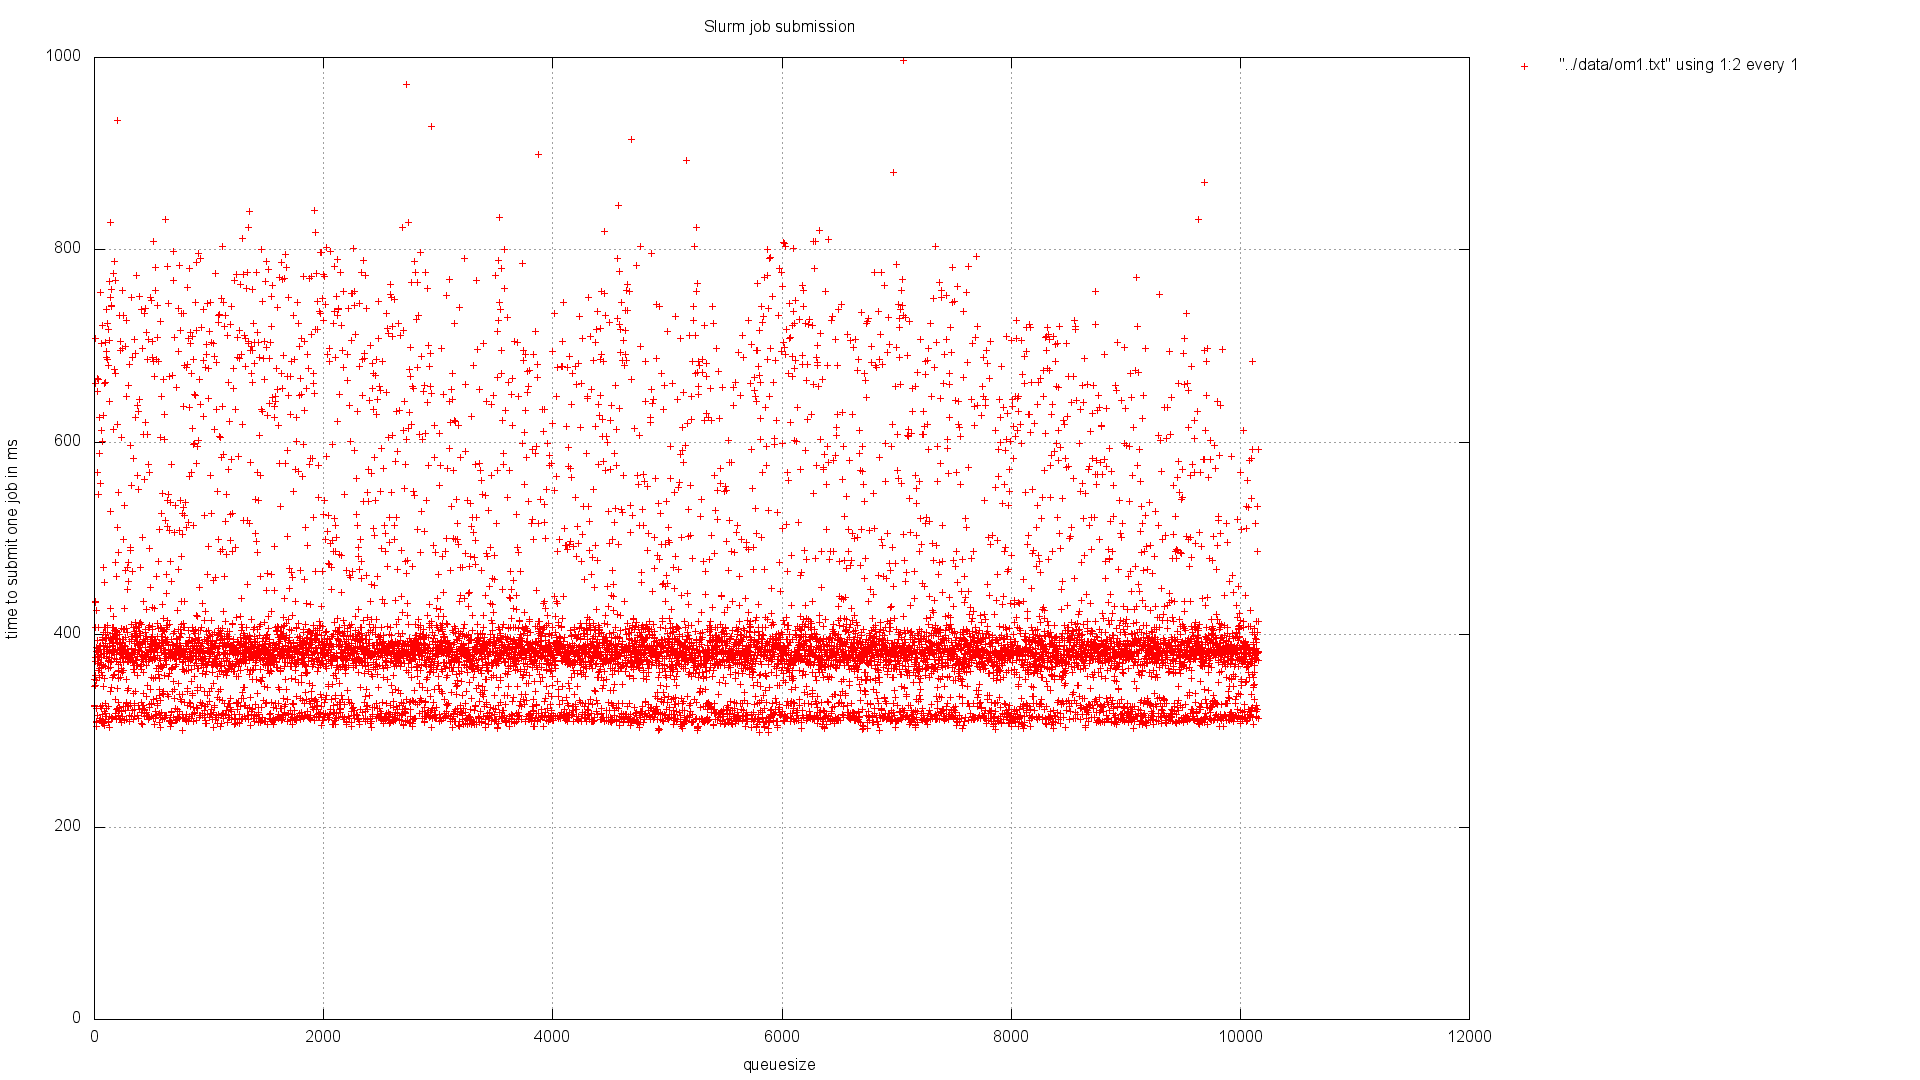
\includegraphics[scale=0.8]{../oar/output/pics/oar.png} 
		\caption{Laufzeit Benchmark[B4]}
	\end{figure}
    Bei OAR liegt die Zeit konstat bei ca. 400 ms unabhängig der Größe
    der Queue, jedoch mit einer relativ großen Streuung.
    \newpage 

	\begin{figure}[H]
		\centering
		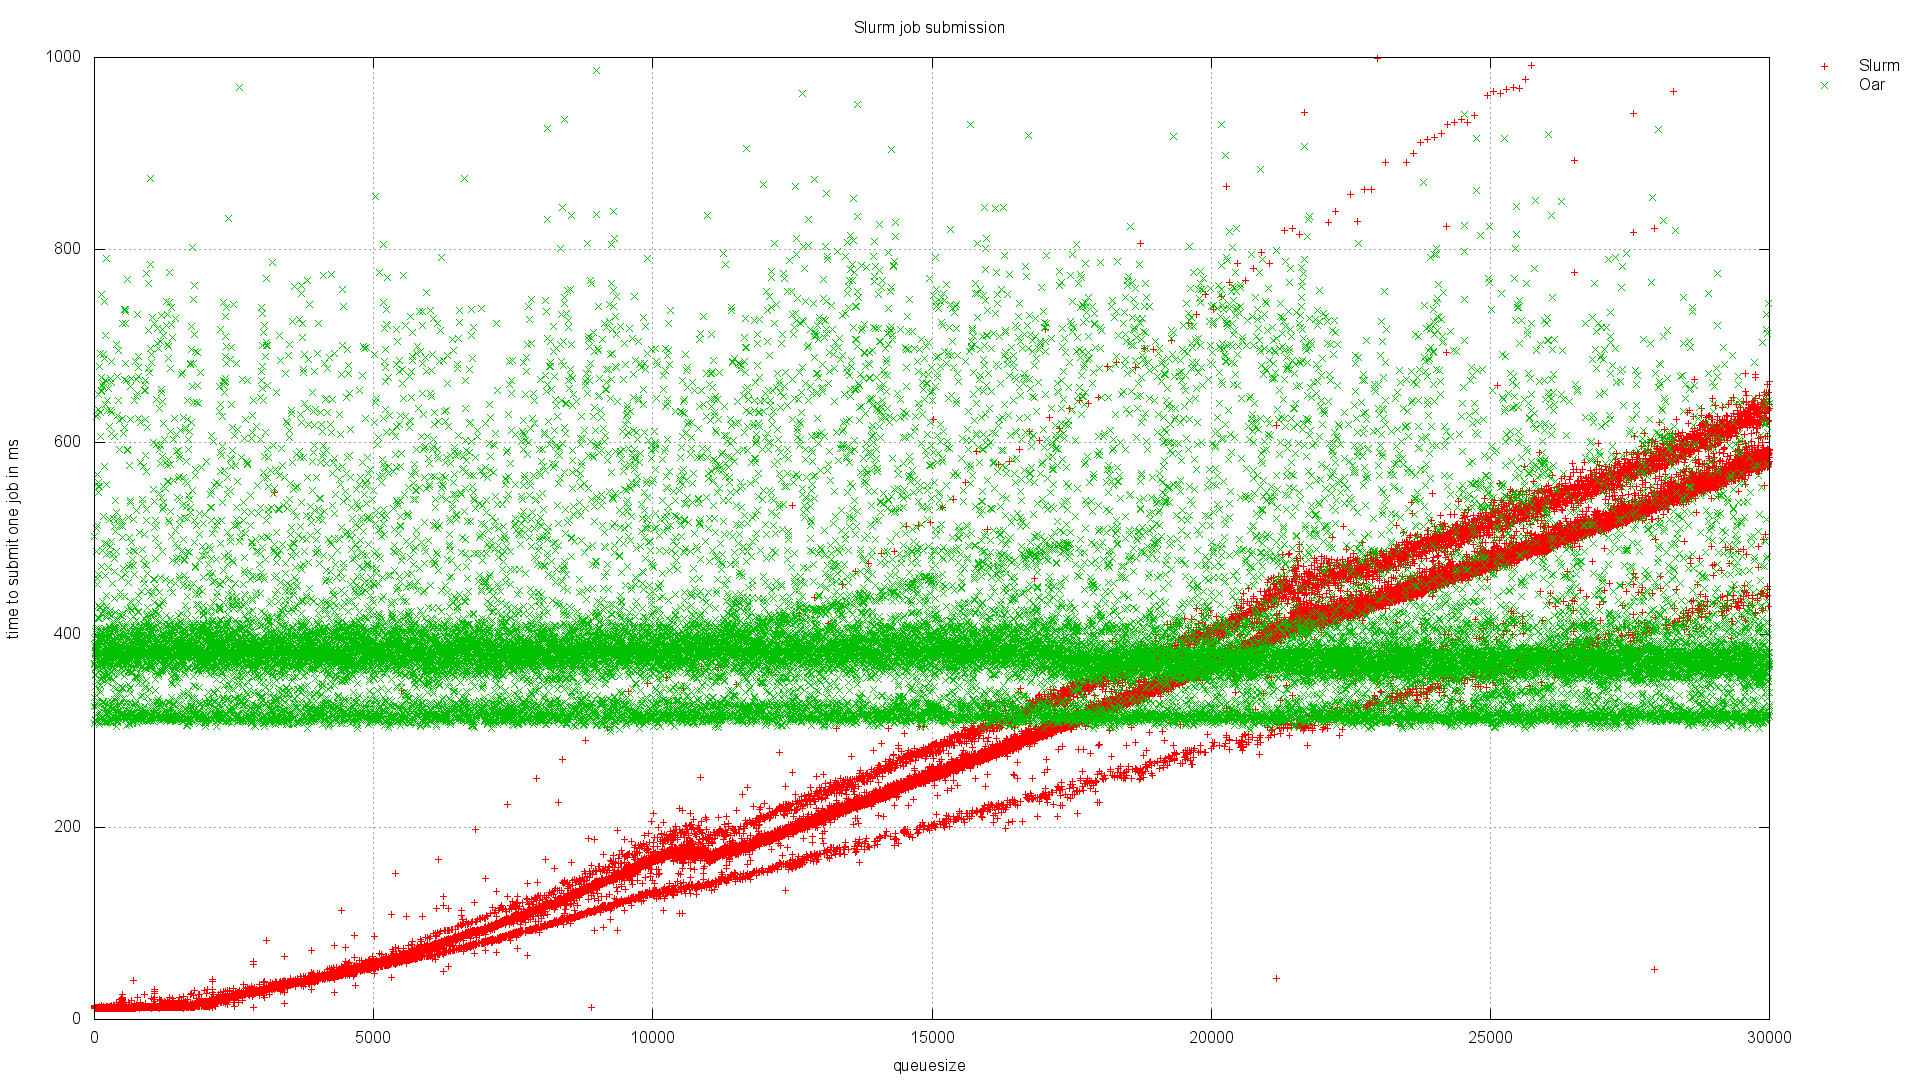
\includegraphics[scale=0.75]{../oar/output/pics/oar_slurm.png} 
		\caption{Laufzeit Benchmark[B4]}
	\end{figure}
    Ab ca. 20000 wartender Jobs ist Slurm bei Submitten neuer Jobs langsamer als 
    OAR. 
    \newpage 

\section{Fazit}
Hinsichtlich der Handhabung für einen durchschnittlichen Benutzer
unterscheiden sich beide Systeme kaum. Slurm und OAR lassen sich mit ählichen
Befehlen bedienen.
Für einen Administrator ist Slurm in den meisten Fällen jedoch 
die geeignetere Wahl.
Da Slurm weiter verbreitet ist als OAR, lassen sich häufiger 
Lösungen zu Problemen finden.

OAR wirbt mit einigen interessanten Features, wie z.B CPUSet, Besteffort queues, etc. , die
jedoch entweder bei anderen Batchsystemen ebenfalls vorhanden sind,
sich durch zusätzliche Plugins verfügbar machen lassen oder aber nur in bestimmten Einzelfällen nützlich sind.
Bei einer oberflächlichen Betrachtung und gewöhnlichen Benutzung kommen diese nicht zum Tragen.

Wenn jedoch sehr viele Jobs auf ihre Ausführung warten müssen, hat OAR mit seiner konstaten submission time einen 
sehr großen Vorteil gegenüber Slurm. Bei einer Jobanzahl von über 100000 wird die Zeitdifferenz signifikant sein und OAR sollte bevorzugt werden.



\begin{thebibliography}{999}
	    \bibitem [0] {} Oar Official Website \url{https://oar.imag.fr}
	    \bibitem [1] {} Oar University of Luxemburg \url{https://hpc.uni.lu/users/docs/oar.html}
	    \bibitem [2] {} Grid5000 Official Website \url{https://www.grid5000.fr}
	    \bibitem [3] {} Slurm Official Website \url{https://computing.llnl.gov/linux/slurm/}
	\newline
\end{thebibliography}
